\documentclass{article}

\usepackage{graphicx}
\usepackage{wrapfig}

\usepackage[utf8]{inputenc}


\topmargin=-0.45in
\evensidemargin=0in
\oddsidemargin=0in
\textwidth=6.5in
\textheight=9.0in
\headsep=0.25in

\title{Lab 2 Writeup - CSE490R}
\author{Tarkan Al-Kazily, Yuta Araki, Dilraj Devgun}
\date{May 2019}

\begin{document}

\maketitle

\section{Introduction}

In this lab, we implemented three different kinds of motion controllers:
a PID controller, a Pure Pursuit controller, and a Model Predictive controller.
This writeup goes over some of the choices we made in tuning these controllers,
and compares their performance.

Along with this writeup we have a large store of videos in the \texttt{videos} folder.
Here are a few of the ones you should watch.
\begin{center}
\begin{tabular}{l|l}
Video & Description \\
\hline
\texttt{sim\_pid.mp4} & Simulation of our PID controller. \\
\texttt{sim\_pp.mp4} & Simulation of our Pure Pursuit controller. \\
\texttt{sim\_mpc.mp4} & Simulation of our MPC controller. \\
\texttt{purepursuit\_real.mp4} & Our Pure Pursuit controller on the real robot. \\
\texttt{mpc\_tuned.mp4} & Our MPC controller on the real robot.  \\
\texttt{mpc\_tuned\_avoid\_wall.mp4} & Our MPC controller avoiding real obstacles.
\end{tabular}
\end{center}

\newpage
\section{PID Controller}

The first controller we implemented was a PID controller, which stands for
Proportional Integral Derivative controller. To reduce complexity for this
lab, we were instructed not to implement the integral gain, making our controller
more of a PD controller.

The initially provided values for $K_p$ and $K_d$ were effective before tuning.
It's performance curve is given in Figure \ref{fig:pid_orig_perf}.
In tuning, we prioritized the controller quickly reaching the set point of the
path (given by the cross track error going to zero) as well as minimizing
the overshoot of the car. We first determined the
$K_p$ gain until our controller would reach the reference path in the
desired time interval (approximately 100 to 150 ms on the plot), ignoring the consequence of
overshooting, and then increased the
$K_d$ gain until the controller no longer overshot the set-point.
Figure \ref{fig:pid_tuneKp} shows the performance of our controller with only
$K_p$ non-zero (tuned to $0.3$) and Figure \ref{fig:pid_tuneKpKd} shows
the performance of the final, tuned controller with both $K_p = 0.4$ and $K_d = 0.3$.
We did end up increasing the $K_p$ after tuning $K_d$ to improve the time it takes
the controller to reach the setpoint.

\begin{figure}[!h]
\centering
  \includegraphics[width=150mm]{images/pid_015_020.png}
  \caption{Original PID performance}
  \label{fig:pid_orig_perf}
\end{figure}

\begin{figure}
  \includegraphics[width=\linewidth]{images/pid_03_00.png}
  \caption{Approximate desired $K_p$ performance (0.3) with $K_d = 0.0$}
  \label{fig:pid_tuneKp}
\end{figure}

\begin{figure}
  \includegraphics[width=\linewidth]{images/pid_04_03.png}
  \caption{Tuned $K_p$ and $K_d$ performance ($K_p = 0.4, K_d = 0.3$)}
  \label{fig:pid_tuneKpKd}
\end{figure}

We found that increasing $K_p$ had the effect of taking sharper
turns towards the set-point, up to a point where the minimum turning radius
of the car was achieved. Increasing $K_d$ would cause the car to straighten out
nearer to the reference path which would reduce overshooting.

As mentioned, our final $K_p$ and $K_d$ values are $K_p = 0.4$ and $K_d = 0.3$.

To implement the derivative computation of our controller, we used
the analytic approach with $\sin(\psi_e)$. In terms of the controller's performance
it does very well at ensuring that as the error decreases and the car
reaches the reference path that the car is pointing in the direction of the
reference path, and won't cross it rapidly. We chose to implement this
first because of its simplicity over numerical differentiation (as it doesn't
rely on tracking previous error values). It also has the benefit that it
isn't as impacted by noise in sampling the error, since using numerical
integration if the samples for the derivative aren't smooth unexpectedly large
derivative terms can negatively impact performance. However, due to time constraints
we did not have time to implement and test numerical derivation methods.

\newpage
\section{Pure Pursuit Controller}

We started with vary short look-ahead distance of 0.1 meters
(the performance for which is given in Figure \ref{fig:pp_01}),
which did not 
work too well as it forced the car to take super sharp turns repeatedly and 
caused car to move in a circular path. From there, we kept increasing the
look-ahead distance until controller was able to get car back on track in 
reasonable manner, which was at 0.9 (see Figure \ref{fig:pp_09}).
We tried higher values for look-ahead, which caused car to cut corners
(see Figure \ref{fig:pp_15} to see the performance of a lookahead of
1.5 meters).
Look-ahead distance less than 0.7 or greater than 1.2 did not perform well 
due to reasons stated above.

\begin{figure}[!h]
  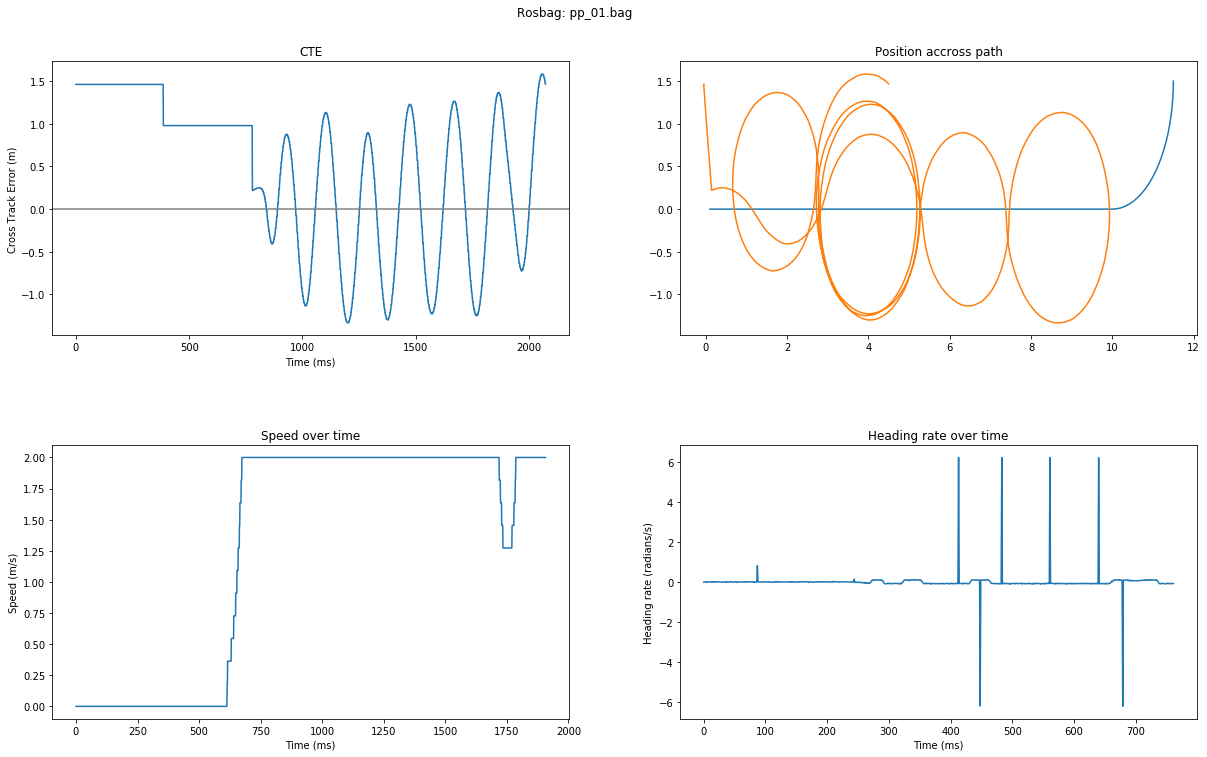
\includegraphics[width=\linewidth]{images/pp_01.png}
  \caption{Pure Pursuit performance with lookahead of 0.1 meters}
  \label{fig:pp_01}
\end{figure}

\begin{figure}
  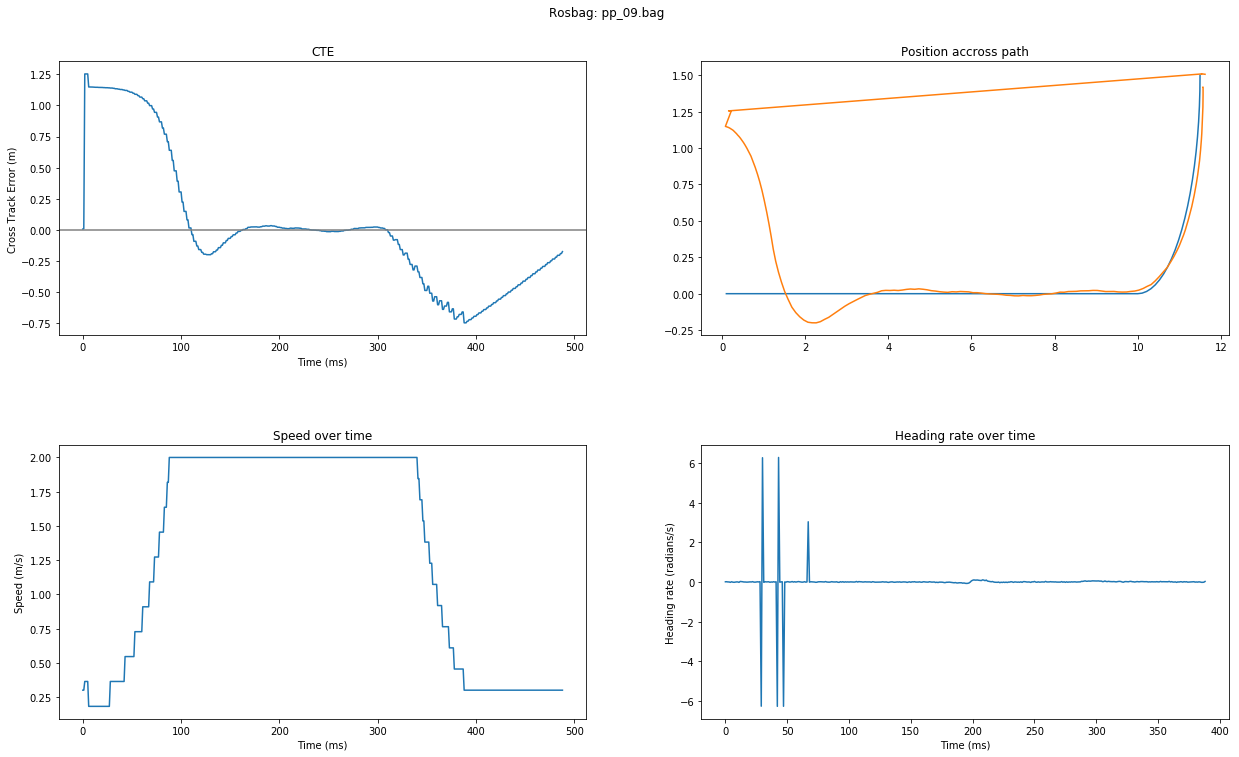
\includegraphics[width=\linewidth]{images/pp_09.png}
  \caption{Final Pure Pursuit performance with lookahead of 0.9 meters}
  \label{fig:pp_09}
\end{figure}

\begin{figure}
  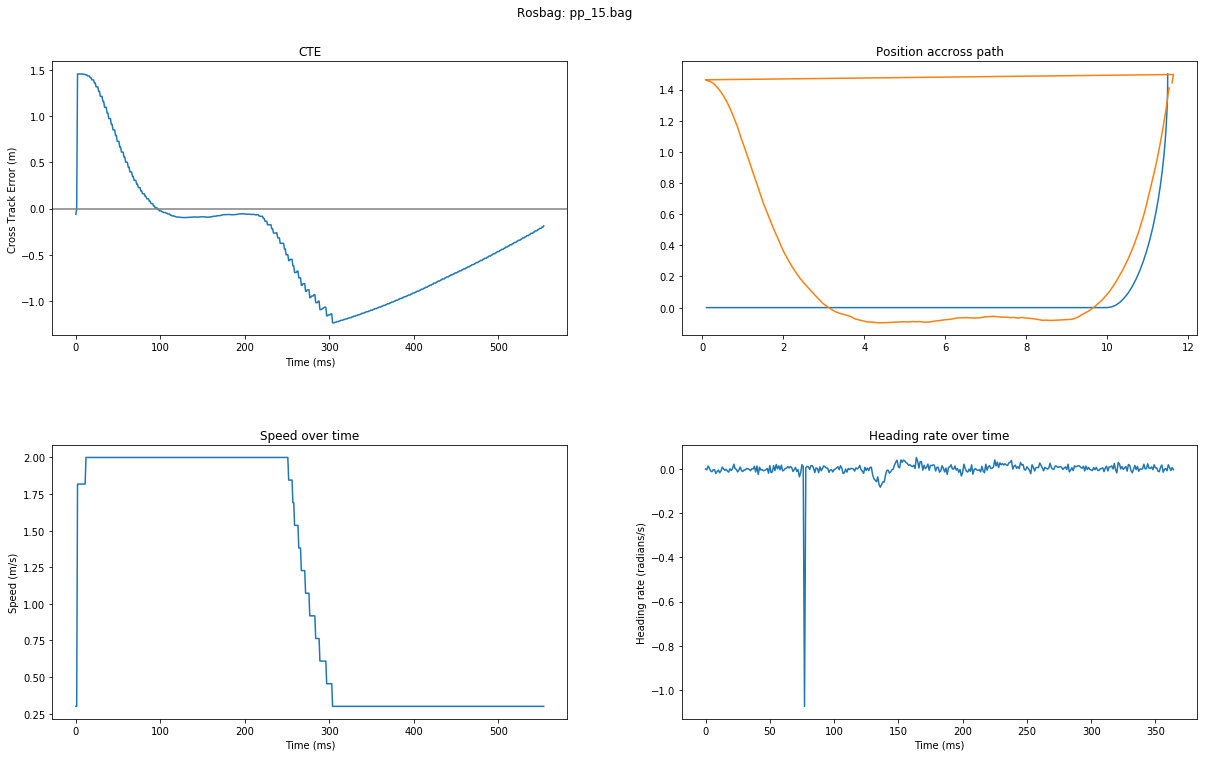
\includegraphics[width=\linewidth]{images/pp_15.png}
  \caption{Pure Pursuit performance with lookahead of 1.5 meters}
  \label{fig:pp_15}
\end{figure}


Varying turning radius of the circle path did not have significant affect 
on the performance of our controller, as long as turn radius on the path 
was larger than car's capability. Testing on various turning radius did 
not necessary help narrowing down the optimal look-ahead distance, 
however, it did help us confirm that look-ahead distance we chose 
was good enough.

Varying the desired\_speed parameter did not affect the performance of 
our controller. Faster speed made the car to overshoot a little but 
there was no significant overshoot. Lower speed made decreased 
the overshooting.

When running the pure pursuit controller on the real robot, we found that
our existing lookahead value worked well and didn't need additional tuning.

Comparing PD controller and Pure Pursuit controller, it seems like 
PD controller is more generalizable and Pure Pursuit controller 
performs better on constant curvature (e.g. circle path).

\newpage
\section{Model Predictive Controller}

A plot of our trajectories and cost function heatmap
is given in Figure \ref{fig:mpc_traj_heatmap}.
Initially we used constant curvature trajectories with minimal variation between
paths due to the simplicity of development, but decided to implement
a variation where after a certain percentage of our actions the steering
angle is set to straight. This change further penalizes paths that put the
car directly in front of an obstacle in the short term because it doesn't assume
that the car will continue to turn as part of the future path planning.

\begin{wrapfigure}{r}{65mm}
  \centering
  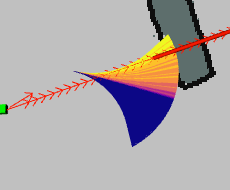
\includegraphics[width=50mm]{images/mpc_traj_heatmap.png}
  \caption{Our MPC Trajectories and Heatmap}
  \label{fig:mpc_traj_heatmap}
\end{wrapfigure}

We began tuning our MPC by testing on the initial parameters for K
and T which caused our robot not to avoid obstacles since we were not 
looking far enough in the future to adjust our planned motion. From this
point we doubled our T by twice to 16 and also again to 32. The results 
for these values were much better, yielding results that we expected 
where the robot would navigate around forthcoming objects. In addition, 
we also ran our simulation using a roll out of 100 which caused our robot to 
search too far into the future which would make us stop early and make too 
harsh of adjustments to what is immediately impending for the robot to navigate. 
The performances of these tests in simulation are given in Figures
\ref{fig:mpc_tune_T_orig}, \ref{fig:mpc_tune_T_16}, \ref{fig:mpc_tune_T_32},
and \ref{fig:mpc_tune_T_100} respectively.

\begin{figure}[!h]
\centering
  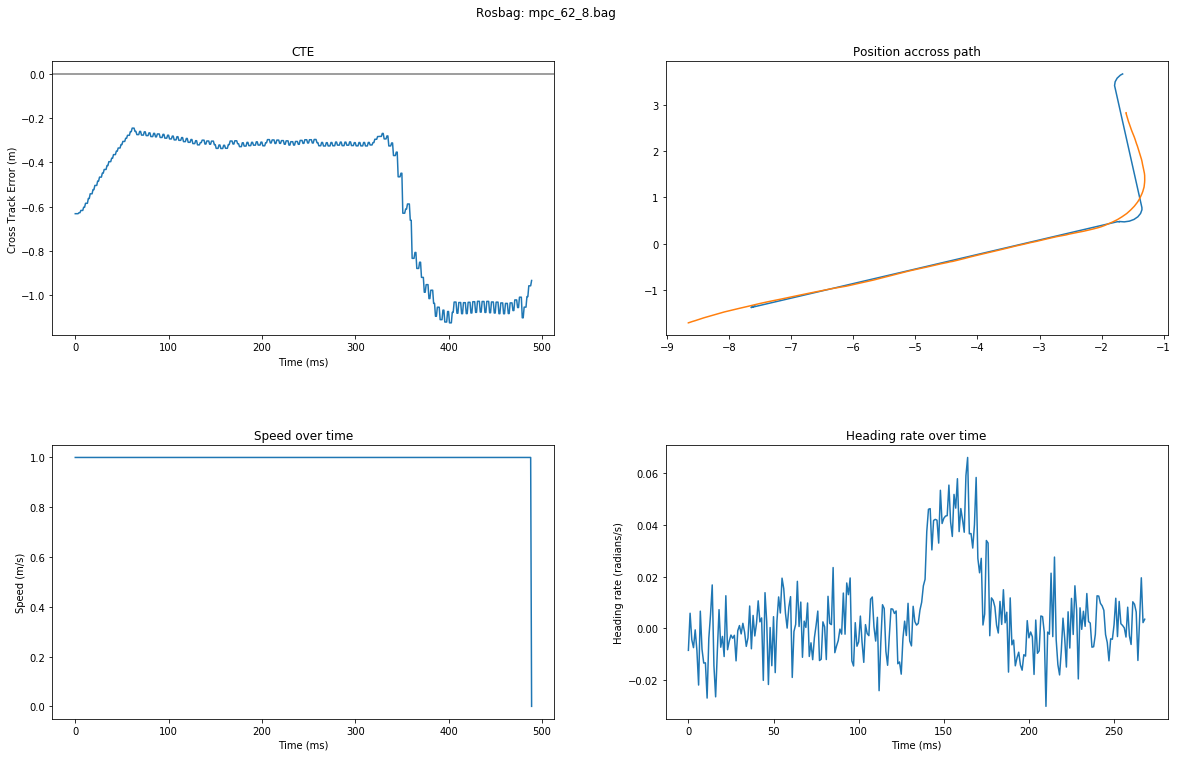
\includegraphics[width=150mm]{images/mpc_62_8.png}
  \caption{Simulated $K$ and $T$ performance ($K = 62, T = 8$)}
  \label{fig:mpc_tune_T_orig}
\end{figure}

\begin{figure}
  \centering
  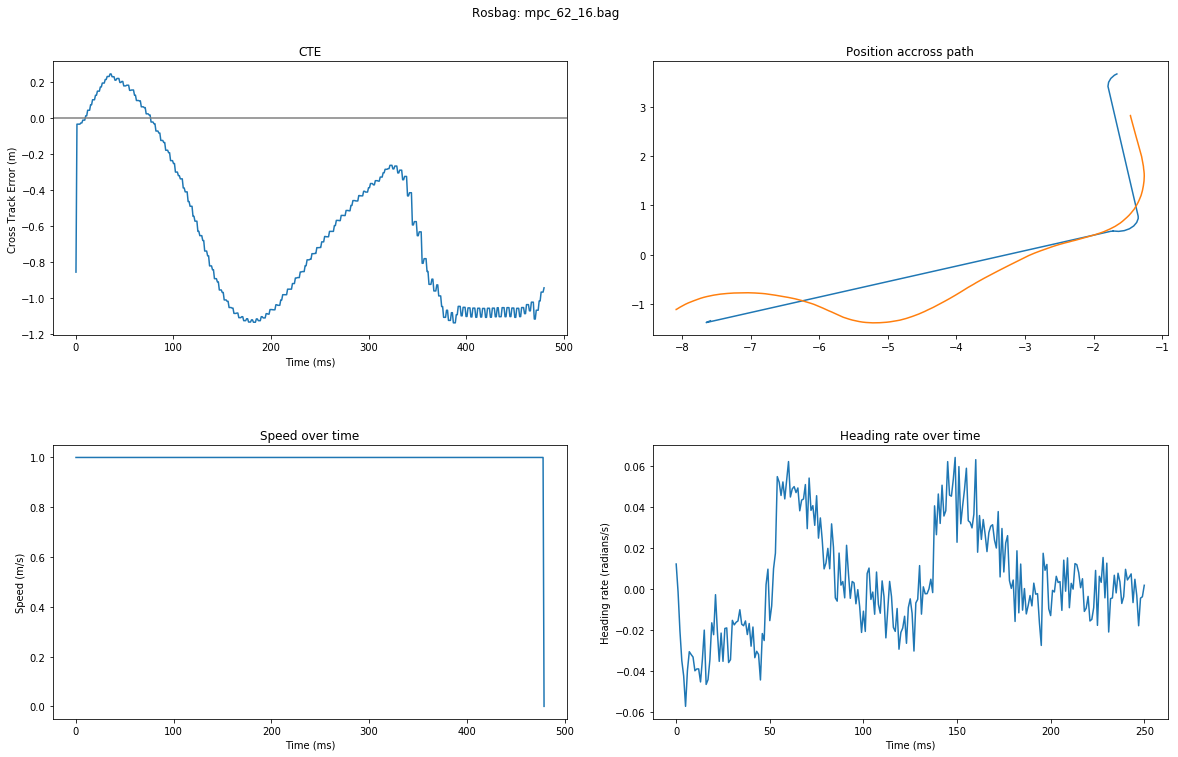
\includegraphics[width=150mm]{images/mpc_62_16.png}
  \caption{Simulated $K$ and $T$ performance ($K = 62, T = 16$)}
  \label{fig:mpc_tune_T_16}
\end{figure}

\begin{figure}
  \centering
  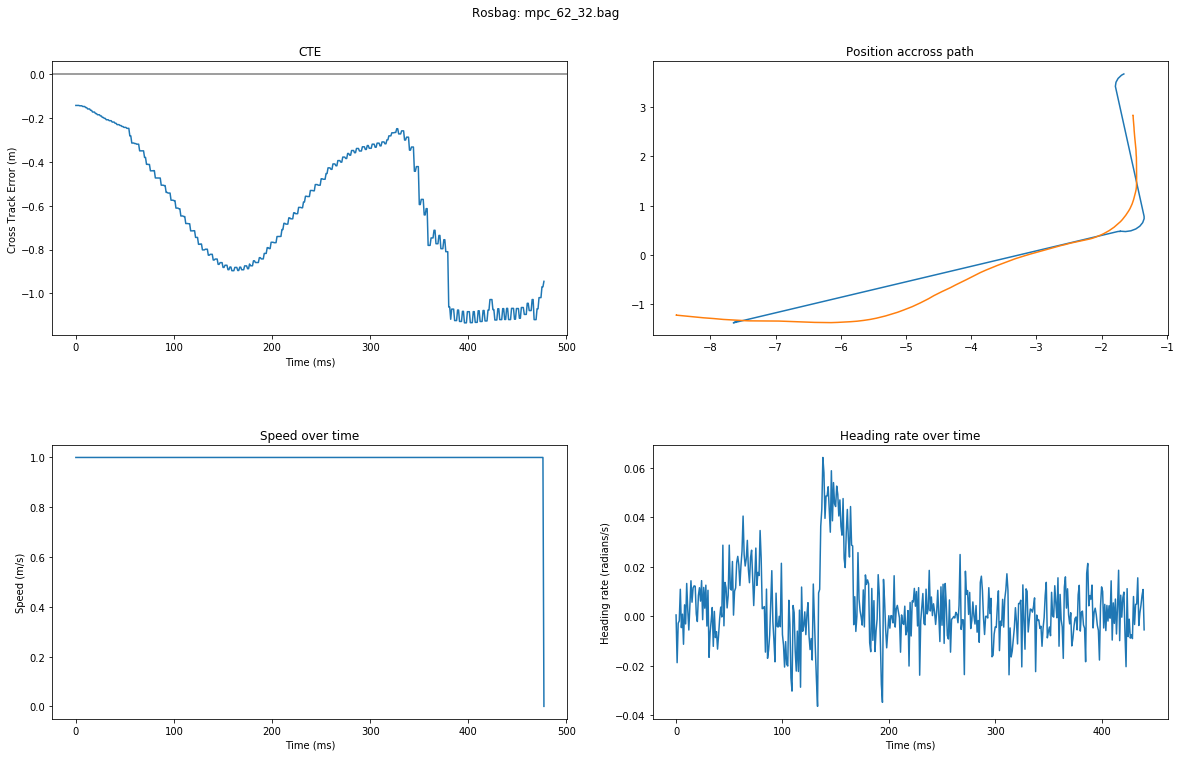
\includegraphics[width=150mm]{images/mpc_62_32.png}
  \caption{Simulated $K$ and $T$ performance ($K = 62, T = 32$)}
  \label{fig:mpc_tune_T_32}
\end{figure}

\begin{figure}
  \centering
  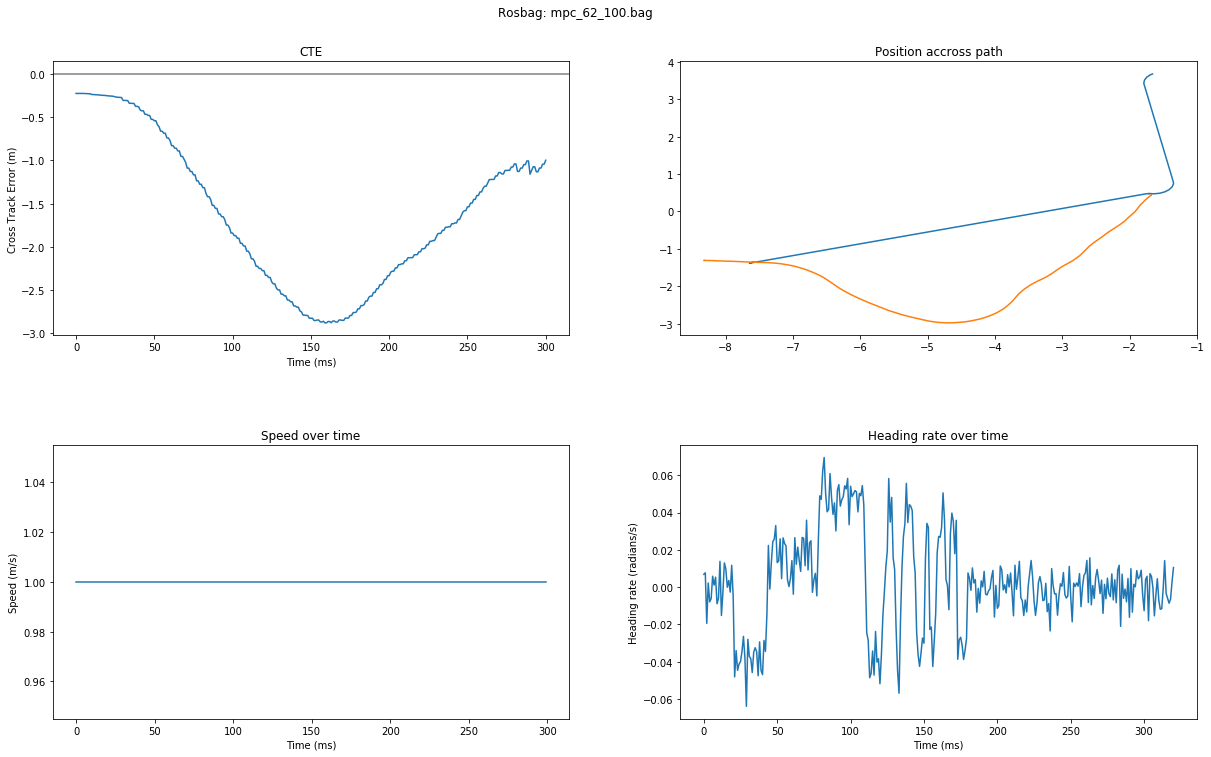
\includegraphics[width=150mm]{images/mpc_62_100.png}
  \caption{Simulated $K$ and $T$ performance ($K = 62, T = 100$)}
  \label{fig:mpc_tune_T_100}
\end{figure}

\newpage
Once we had a strong initial value for $T$, we tested it on the real
robot to avoid the cabinet in CSE 022. We found that with the default
cost function having such a high $T$ value (32) was problematic
with the existing $dt$ parameter (which was in timesteps of .1 second).
We experimented with smaller $T$ values, but as part of tuning on the
real robot found that the $dt$ value was better in smaller timesteps,
finally choosing $dt$ to be 0.4 seconds. With this we increased $T$
to have the similar rollout distance as before. We also increased $K$
to guarantee a greater density of poses further from the current pose.
Our final $T$ and $K$ values are 60 and 150 respectively.

Finally, we experimented slightly with our cost function, with a focus
on tweaking the collision weight so that it would reliably avoid
obstacles in the real. Initially we tried increasing
the collision weight by a factor of 10, and found that resulted in the
robot avoiding the path too much. A weight of $5 \cdot 10^5$ was more
appropriate when equally distributed over all the collision poses.
We finally implemented a scaled weight distribution that more heavily
penalizes collisions for rollouts fewer timesteps from the current pose.
This had a very positive effect on our car's avoidance performance,
and reduced the case where paths that extended beyond the other side
of the obstacle were not penalized enough. It did require tuning our
scaling factor properly, along with the overall collision weight,
which we did by trying to increase these values until the car
would more reliably avoid obstacles.

For the lookahead principle, we used the same method as in our PID
controller, in which we found our next waypoint by finding the closest
waypoint and then returning the waypoint that is the lookahead distance
in front of that point. This is similar in concept to Pure Pursuit's
lookahead principle, but uses the lookahead distance from the reference
pose closest to our current pose, as opposed to the distance from
the current pose.

\newpage

\section{Overall Findings}

The PID controller was best on straightaways, but did adequately
on turns with small curvature, since its $K_p$ gain would be enough
to make it turn consistently. We believe that if we added an integral
term to the PID controller that it would more closely follow a circular
reference path, since over time the integral term would be able to correct
for the negative feedback of the derivative factor.

The Pure Pursuit controller worked best on large, consistent turns such
as the circle reference path, which makes sense due to the controller's
inherent assumption that all motion the car makes travels in a circle.
It would often oscillate on straight-aways more than other controllers,
but could operate faster than the other controllers.

The MPC controller stood out as the most generalizable controller
among our choices, and did well regardless of the scenario. We 
believe this is due to the generalizability of optimizing the cost of
multiple paths as part of planning each control action. It has the
obvious strength that it can adapt its path in the presence of minor
obstacles on the path. It was the most robust to failures because of
this, easily returning to the path if it over shot or avoided an obstacle.

All our controllers performed well in the sim-to-real transition,
but there was definitely some discrepancy. Our PID controller was
one of the weakest, because the real car's response behaves differently
from the simulation, and therefore requires more tuning to
overcome factors not present in the simulation. An integral term
would also help here, as we noticed that the settle point of
the PID controller was not directly on the reference path.
The pure pursuit transitioned to the real world the best.
Finally, our MPC controller took a lot of tuning in the real world
to choose more effective $K$ and $T$ values for the real world case.

\end{document}

